\section{Silicon Photomultiplier}
In order to correctly identify and tag background events, the light detection of the \ac{sbt} has to provide accurate timing information.
Therefore \acp{sipm} were chosen as photodetectors.
These photodetectors consist of up to thousands of pixels.
Each pixel is a photodiode with a typical edge length between \SI{10}{\micro\meter} and \SI{100}{\micro\meter} \cite{nucl}.
If triggered by light, a \ac{sipm} sends out a charge signal proportional to the incoming light.
This charge possesses a fast-rising edge with a rise time of the order of tens of \si{\piko\second} \cite{nucl}.
Besides the good time resolution, \acp{sipm} also make it possible to count the arriving photos with a sensitivity down to single photons \cite{HAMA_mppc}.


Similar to every photodiode, \acp{apd} utilize the photoelectric effect, to generate an electric charge signal in response to a light signal.
This is made possible by using silicon as a base material and introducing impurities. 
This process is called doping and there are two different possibilities for doping. 
In the n-doping, the impurities are atoms with five valence electrons.
Four of these electrons are part of boundings with silicon atoms, and the fifth electron is only weakly bound.
When p-doping, atoms with only three valence electrons are inserted into the silicon.
This leads to missing charges in the silicon, called holes.
By having an n-doped and a p-doped region in the silicon, the excess electrons from the n-doped region combine with the holes from the p-doped region, resulting in a depleted region at the pn-junction.
If a photon hits the photodiode, it can create an electron-hole pair, or $eh$-pair.
The electron and the hole get split by the electric field and thus create a charge signal.
In order to increase the sensitivity of the photodiode, an intrinsic layer can be added in between the two doped regions, thus increasing the depletion layer and therefore the photosensitive area.
Such a photodiode is called a pin-diode.
An \ac{apd} with a weakly doped $\pi$ intrinsic layer and strongly doped $p^+$ and $n^+$ layers is shown in \autoref{fig:pin_diode}.
This intrinsic layer can either be not doped at all or weakly doped.
In the case of \acp{apd} the intrinsic layer is weakly doped. 
In order to amplify the signal, a strong doped region is inserted, thus creating a multiplication zone.
\begin{figure}
	\centering
	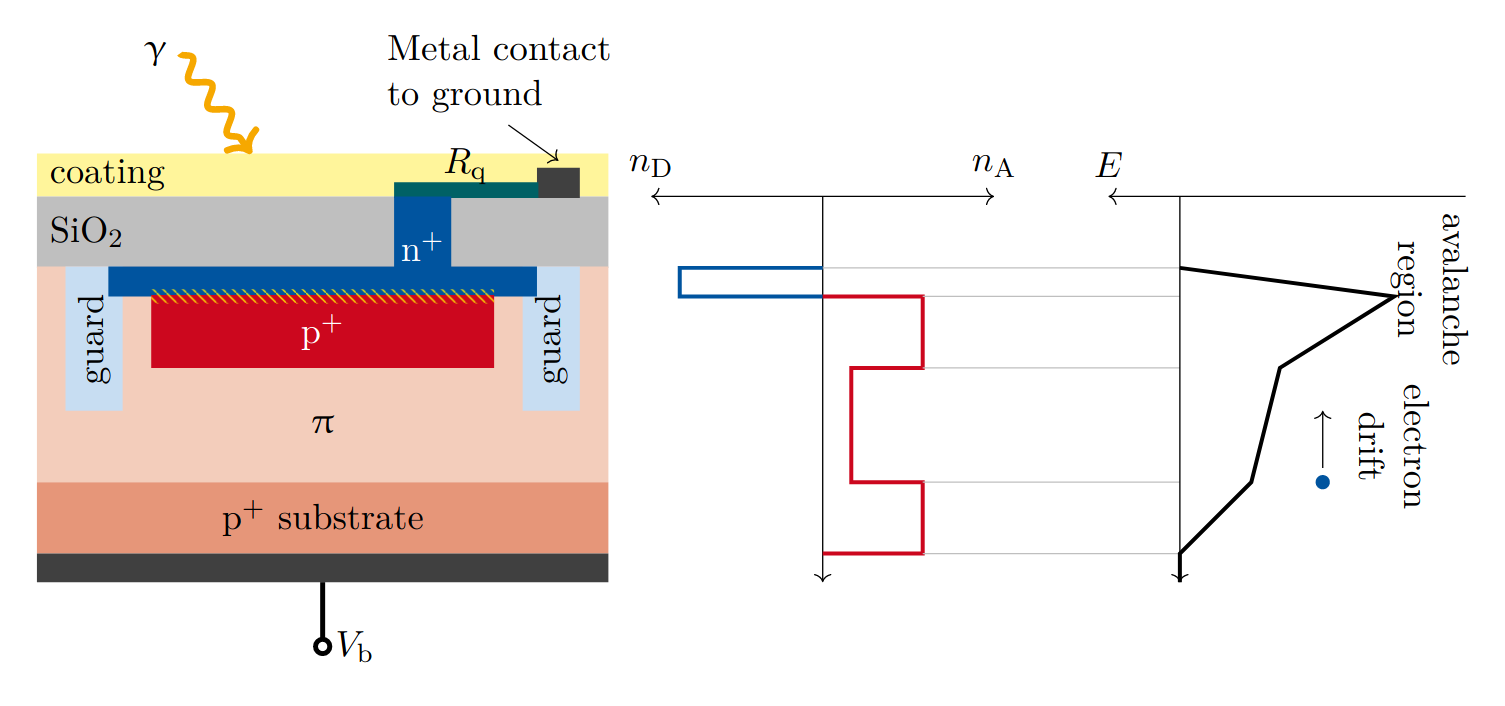
\includegraphics[width=1.\textwidth]{pictures/pin_diode}
	\caption[Illustration of a APD.]{Composition of a avalanche photo diode with the bias voltage $V_\text{B}$ applied in reverse direction. Between the contact to ground and the strongly doped $n^+$ layer is the quenching resistor $R_\text{q}$ connected in series. Next to the $n^+$ layer is a strongly doped $p^+$ layer. In the region of these two layers is the electric field, shown on the right figure, the strongest. There a electron or hole can initiate an avalanche. After the $p^+$ layer comes a intrinsic weakly doped $\pi$ layer. This layer increases the sensitive volume of the diode. If a electron-hole pair is created and seperated by the electric field. The hole drifts towards the multiplication region and can start an avalanche. The next layer is a $p^+$ layer which connects to a metal connector and high voltage. \cite{kemp}}
	\label{fig:pin_diode}
\end{figure}

When a reverse bias voltage is applied to the \ac{apd}, the electric field between the $n^+$ and $p^+$ layers is strong enough that a created $eh$-pair creates more $eh$-pairs, resulting in an avalanche.
For this avalanche process to be possible the reverse bias voltage must be at or above the breakdown voltage of the \ac{apd}.
With such a bias voltage applied, the \ac{apd} operates in the Geiger mode and the avalanche is then self-sustaining.
This results in a macroscopic signal and makes the detection of single photons possible.
Therefore these diodes are also called \ac{spad}.
To stop the avalanche, a quenching resistor is connected in series with the \ac{spad}.
With an increasing current signal flowing through the quenching resistor, the voltage drop at this resistor increases, and thus the bias voltage at the \ac{spad} decreases.
When the bias voltage drops under the breakdown voltage, the avalanche is no longer self-sustaining and stops.
Thus the signal amplitude of a \ac{spad} is always similar, independent of how many photons arrive at the same moment.
In \acp{sipm} hundreds to thousand \acp{spad} are connected in parallel, each with a high resistance quenching resistor in series. 
Usually, the \ac{spad} pixels are placed in a rectangular form with an edge length of a few \si{\milli\meter}.
\autoref{fig:sipm_closeup} shows a picture of a \ac{sipm} and one picture of a single pixel of a \ac{sipm}.
Due to the property of the \acp{spad} that the output signal is always similar for each \ac{spad}, the output signal of a \ac{sipm} is the output signal of one \ac{spad} multiplicated with the number of triggered \acp{spad}.
Therefore, if the number of photons arriving simultaneously at a \ac{sipm} is low enough, that the probability of one \ac{spad} being hit by two or more photons is low, one can count photons with a \ac{sipm}.
This and the relatively low cost, high durability, and impassivity to magnetic fields make them a good option for photodetection for the \ac{sbt} and similar detectors.

In the following different properties of \acp{sipm} are presented, beginning with the signal shape of a single \ac{spad} and of a \ac{sipm}.


\paragraph{The signal shape} of a \acp{spad} starts with a fast exponential rise with the time constant 
\begin{align}
	\tau_\text{rise}&=R_\text{S}\cdot C_\text{d}
\end{align}
with the resistance $R_\text{rise}$ and capacitance $C_\text{d}$ of the \ac{spad} \cite{HAMA_mppc}.
After the signal reached its maximum current at around 
\begin{align}
	I_\text{max}&\approx \frac{V_\text{ov}}{R_\text{q}}
\end{align}
the quenching and recharging of the \ac{spad} starts.
Thus the current signal decreases again exponentially.
The time constant for the signal decay
\begin{align}
	\tau_\text{decay} &= R_\text{q}\cdot C_\text{d}
\end{align}
depends on the capacitance $C_\text{d}$ of the \ac{spad} and the quenching resistor $R_\text{q}$ \cite{HAMA_mppc}.
This signal develpment is shown in \autoref{fig:spad_signal_shape}.
\begin{figure}
	\centering
	\includegraphics[width=0.75\textwidth]{pictures/spad_signal_shape}
	\caption[SPAD signal shape]{Single photon avalanche diode signal shape. The exponential rise with the time constant $R_\text{S}\cdot C_\text{d}$ is followed by the exponential decay with the time constants $R_\text{q}\cdot C_\text{d}$. The maximum of the current signal is at approximately $V_\text{ov}/R_\text{q}$ \cite{HAMA_mppc}}
	\label{fig:spad_signal_shape}
\end{figure}

When multiple \acp{spad} in a \ac{sipm} are triggered, the output signal will be the summation of the signals from all triggered \acp{spad}.
Besides the number of triggered \acp{spad}, the time difference between the signals from the single \acp{spad} influences the signal.
In the case, that all \acp{spad} are triggered at the same time, the \ac{sipm} signal will have the shape of a \ac{spad} signal scaled up by the factor of the number of triggered \acp{spad}.
If the signals form the individual \acp{spad} have a small difference in time, the \ac{sipm} signal will become broader.




\paragraph{The gain} $G$ of a \ac{sipm} describes the number of charge carriers released in each avalanche.
Due to the quenching, this parameter is well defined \cite{}.
It can be calculated from the applied voltage $U_\text{bias}$, the breakdown voltage $U_\text{bd}$ and the capacitance $C_\text{d}$ of a \ac{spad} with
\begin{align}
	G &= \frac{(V_\text{bias}- V_\text{bd})\cdot C_\text{d}}{\text{e}}.
\end{align}
Here e represents the charge of one electron.
Usually the gain is in the order of $10^5$ to $10^7$ \cite{nucl}.

\paragraph{The noise} in \acp{sipm} can be sorted into two categories.
The first is primary noise, it describes the triggering of avalanches by thermaly created $eh$-pairs and not by incident photons.
Because the rate of theses thermaly caused events increases and decreases with the temperature, by controling the temperatur one can influence and decrease the rate of primary noise events.
The second category is the correlated noise.
It includes all events triggered by a primary event.
This correlated noise does have two causes.
One cause is the trapping and releasing of charge carriers from the avalanche. 
When the time between the trapping and releasing is long enough, the avalanche of the primary event stoped and the released carrier can trigger another avalanche.



\subsection{Photoelectron spectrum}


After the theory and important properties of \acp{sipm} are now introduced, the next chapter will present the measurement setup and data acquisition used for this thesis.
